\documentclass{article} % For LaTeX2e
\usepackage{nips13submit_e,times}
\usepackage{hyperref}
\usepackage{url}
\usepackage{graphicx}
\usepackage{wrapfig}
\usepackage{caption}
\usepackage{subfig}

\captionsetup{
  font=footnotesize,
  justification=raggedright,
  singlelinecheck=false
}

\title{Banishing the Bid Bot: Detecting Online Bidding Fraud in Facebook Auctions}

\author{
Team: Random Clique \\
Daniel Geng (504588536), Meghana Ginjpalli (804588573), Sara Melvin (004590481), \\
Sonu Mishra (604590548), and Andrew Wong (104036702) \\
Winter 2015
}

\newcommand{\fix}{\marginpar{FIX}}
\newcommand{\new}{\marginpar{NEW}}

\nipsfinalcopy % Uncomment for camera-ready version

\begin{document}

\maketitle

\begin{abstract}

stuff

\end{abstract}

\section{Motivation}

Facebook is a popular online social media platform connecting users from all around the world.
With this efficient form of communication, businesses are able to reach out to their existing customers as well as advertise to new customers by specifying which group of users they would like to advertise to.
Although Facebook can provide space on both their website and mobile site, there is limited webpage ``real estate".
Therefore, Facebook sets up auctions for businesses to bid on designated spaces for advertisement purposes.

Online shopping and bidding are quickly becoming a major proportion of retail transactions. % cite [1]
Consumers are increasingly enjoying the convenience and selection provided by the e-commerce platforms available today.
Unfortunately, legitimate users are being frustrated by bots as they bid at the last possible second.
Automated bids from bots are unfairly able to submit bids almost instantaneously, making it difficult for legitimate buyers to win auctions.
According to a paper released by eBay, 65\% of sessions each day are initiated by bots. % cite [2]

``Facebook Recruiting IV: Human or Robot?" was a past Kaggle Competition that ended in June 2015.
The competition tackles the problem of bot detection in online auction sites.
Our goal is to detect bot-user anomalies in an e-commerce environment using binary classification. 

\section{Background}

Existing approaches have been implemented in order to determine pattern detection for identifying anomalous users.
There are many platforms relying on crowdsourcing for promoting products and services.
However, there are bots pretending to be humans which lowers the consumers? trust in these sites.
Thus, there is a lot of motivation for these companies to have some type of anomaly detector for removing these bots.
These approaches are group-based, temporal-based, and edge attribute graph-based.

\subsection{Group-based Approach}

This approach aims to detect groups of anomalies based on features across multiple users.
Previous methods have attempted to classify based on the similarity of feature groups. % cite [3]
Other methods detect group based anomalies by determining groups based on closeness of certain features, and then determining which groups are anomalous. % cite [4]
The benefits of using these group-based approaches is that it uses the sheer amount of data provided to its advantage.
Generally, however, these approaches assume a static model for the data.
Additionally, due to the large amount of data processed by these approaches, the methods are computationally expensive.

\subsection{Temporal-based Approach}

Unlike some of the other approaches, this method uses only one feature to detect bot-users? suspicious activity.
The temporal-based approach operates under the assumption that the time between user events for bots is significantly different behavior than normal users. %cite [5 6 7 8]
This assumption holds in most situations.
However, bots could be compromised users, which camouflages the anomalous temporal feature(s) with their human host.
Therefore, other features may need to be used for improved detection of bot-users.

\subsection{Edge-attributed Graph-based Approach}

Conventional graph-based approaches observe topological patterns of relations between entities (i.e. users, products, etc), but do not leverage the edge-attributes.
[9] utilizes more features by representing the relationship between entities as an edge-attributed multigraph. % ????
Given the distribution of various clusters of benign user behavior, the information required to describe the behavior of a new user is found in terms of its minimum description length (MDL) from the clusters.
The MDL is used to compute how suspicious a certain user is.
The strength of this approach, however, relies on the rating relationship between users, products, and buyers.
In the project?s bidding data, a seller and rating information is not disclosed, which potentially weakens the applicability of this approach.

\section{Methods}

Various anomaly detection algorithms are compared and contrasted, including BIRDNEST, EdgeCentric and classic machine learning algorithms such as K-means, logistic regression, kernel SVM, naive Bayes, and decision trees to discover bot-anomalous behavior.
Additionally, these models are compared to the model implemented by the winner of this Kaggle Competition, Small Yellow Duck.
Because the dataset from Kaggle (\url{https://www.kaggle.com/c/ facebook-recruiting-iv-human-or-bot/data}) provides labeled data, we are focusing on using supervised algorithms for detection.
We plan to use k-fold cross validation and tune our hyperparameters evaluation metrics. 

To evaluate the efficacy model, we will apply the trained model to our testing data and compare the classifying algorithms based on performance.
The metrics we will use to evaluate the performance of our algorithms is the area under the ROC curve. 

\section{Data}

The data provided includes timestamps of bids, merchandise categories, bidding devices, countries of bids, and the reference URL for a bid.
We plan to use these features and state-of-the art anomaly detection algorithms to determine which method will best identify bot-users.

The bidder dataset contained approximately 2,000 instances and had the following features: bidder\_id, payment\_account, address, outcome.
The bid dataset contained approximately 7.6 million instances and had the following features: bid\_id, bidder\_id, auction, merchandise, device, time, country, ip, url.

The training data set provided by Kaggle had labels for each user, classifying each individual as a human or a bot.
However, the testing data had no labels; therefore, only the training data set could be used for training, validation, and testing.

The training data set was joined with the bids data set, resulting in over 3 million bids.
Overall, it contained 1,984 distinct bidders with 103 of the total users classified as bots.

\section{Software Tools}

Python was used for a majority of our data processing, given the large number of libraries that are publicly available.
Sklearn has a number of built-in machine learning algorithms.
Numpy is very useful for working with matrices and different feature vectors.
Pandas has a high performance data analysis tool used to analyze large amounts of data.
Matplotlib facilitates data visualization, which will yield insights into how our data are related.
Additionally, Python has APIs for Apache Spark and Hadoop, which may prove useful for large-scale data processing.

MATLAB was also used, as a large number of existing state-of-the-art methods have source code written in MATLAB.

\section{Results}

\subsection{Kaggle Winner: ``Small Yellow Duck"}

The second place winner of this Kaggle Competition goes by the name Small Yellow Duck.
Her classification model takes the average of the probabilities predicted by five instances of the Random Forest Classifier.
Random Forests are an ensemble learning method that constructs multiple decision trees in order to create a stronger classification model.

Small Yellow Duck first makes a couple of observations before implementing feature extraction.
First, human bidding activity tends to peak daily as seen in the figure below.
Over the course of three days, there are three peaks where human bidding activity is higher.
This may be because of auctions ending at the same time everyday.

\begin{figure}[h]
\centering
\captionbox{Daily peaks of human bidding activity}{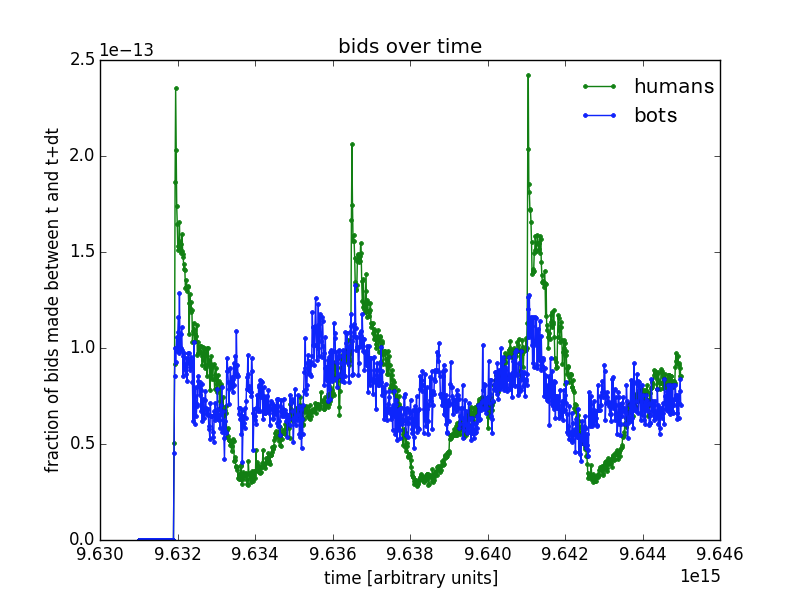
\includegraphics[scale=0.26]{img/yellowduck1.png}}
\end{figure}

Another observation that she made is that auctions tend to last for longer than two weeks.
In this timeframe, robots do not place any bids between 11 to 14 days before the auction ends.
In the figure below, the auction runs for approximately 17 days.
For some reason, between days 11 and 14, human bidding commences while bots tend to keep silent in this duration.

\begin{figure}[h]
\centering
{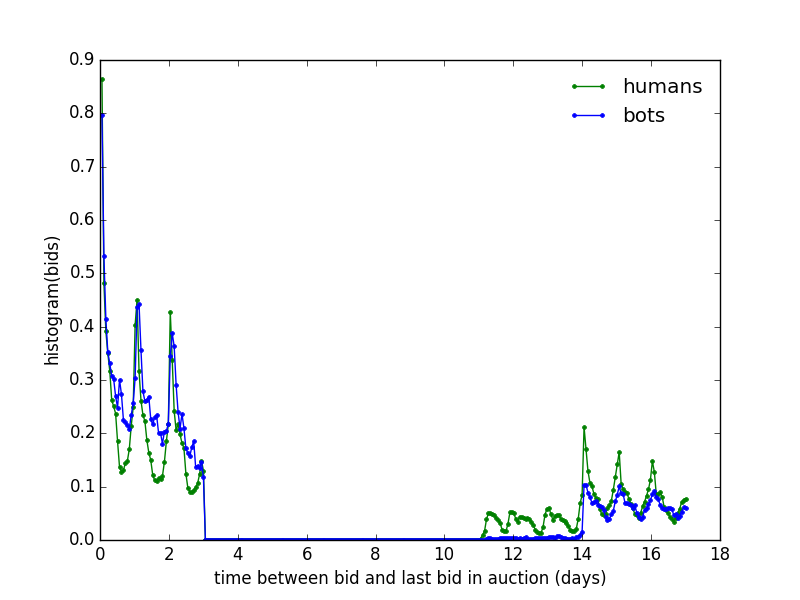
\includegraphics[scale=0.26]{img/yellowduck2.png}}
\end{figure}

The final observation which leads to the feature extraction is that bots tend to bid fast and frequently.
From this, Small Yellow Duck decided that it would be important to have two main features: the median time between user?s bid and user?s previous bid and mean number of bids a user made per auction.
Other features that she decided to use included: entropy for how many bids a user placed on each day of the week, max number of bids in a 20 min span, total number of bids placed by user, average number of bids a user placed per URL, number of bids placed by the user on each of three weekdays in the data, and min and median times between a user?s bid and previous bid by another user in the same auction.

In order to evaluate her results, Small Yellow Duck does cross validation with 100 different training and validation splits where 80\% was training data and 20\% was validation data.
In terms of runtime, training and predicting takes around 3 minutes while 100-fold cross validation takes around 20 minutes.
As a result, the AUC score tends to average at 0.94167.

\subsection{Classic Machine Learning Approaches}

filler

\subsection{BIRDNEST}

\section{Discussion}

\begin{thebibliography}{123}


\end{thebibliography}

\end{document}